\chapter*{Цель и задачи}
\addcontentsline{toc}{chapter}{Цель и задачи}
\label{ch:intro}

\textbf{Цель}: Получение знаний о генераторах случайных величин и
их практической реализации. Работа также закрепляет практические навыки
применения теории вероятности и основ статистического анализа. \\
\\\textbf{Задачи}:

\section*{Задание к лабораторной работе}

\begin{enumerate}
    \item Создайте \texttt{.m} файл в MATLAB и постройте алгоритм, который будет рассчитывать выборочные значения случайной переменной, заданной законом распределения соответственно вашему варианту (варианты задания представлены в таблице 2.1 в конце описания работы). Обратите внимание, что в таблице указаны формулы для плотности распределения. Для применения метода обратных функций необходимо сначала получить функции распределения, что можно сделать путем взятия интеграла от плотности распределения (на бумаге или при помощи специальной функции MATLAB).
    
    \item Сгенерируйте три выборки случайной величины следующих размеров: $N = 50$, $N = 200$, $N = 1000$.
    
    \item Рассчитайте точечные оценки среднего, дисперсии и среднеквадратического отклонения (СКО).
    
    \item Рассчитайте интервальные оценки среднего и дисперсии для уровней значимости $\alpha$: $0.1$, $0.05$ и $0.01$ (всего 18 чисел для среднего и 18 чисел для дисперсии).
    
    \item Сведите все результаты, полученные в пунктах 3 и 4, в таблицы и сохраните их для отчета.
    
    \item Постройте гистограммы, описывающие закон распределения случайной величины по каждой из трех выборок. Для построения гистограммы необходимо разделить интервал, на котором распределена величина, на заданное количество подынтервалов, и рассчитать количество попаданий сгенерированных значений величины в полученные подынтервалы. Высота гистограммы на каждом из подынтервалов определяет количество попаданий. Рекомендуется брать подынтервалы одинакового размера. Для расчета подходящего числа интервалов на гистограмме используется формула:
    \[
    k = \left\lfloor 1 + 3.2 \cdot \ln(N) \right\rfloor
    \]
    где $k$ — число интервалов, $N$ — величина выборки.
    
    \item Постройте поверх каждой гистограммы график теоретической плотности распределения вероятности.
    
    \item Создайте отдельный график, на котором постройте вместе теоретические функцию распределения вероятности и плотность распределения вероятности.
    
    \item Сделайте выводы по полученным результатам (0,5 страницы).
    
    \item Повторите шаги 1–9 для дискретно распределенной случайной величины, учитывая, что некоторые шаги потребуют других вычислений (варианты законов распределения представлены в таблице 2.2). При построении гистограммы для дискретной переменной поместите теоретически заданный и эмпирически полученный законы распределения на одном графике. Если дискретная случайная величина распределена на интервале, равном бесконечности, гистограмму строят для первых 20–30 значений.
    
    \item Сделайте выводы по лабораторной работе (0,5 страницы) и подготовьте отчет.
\end{enumerate}

\begin{figure}[ht]
    \centering
    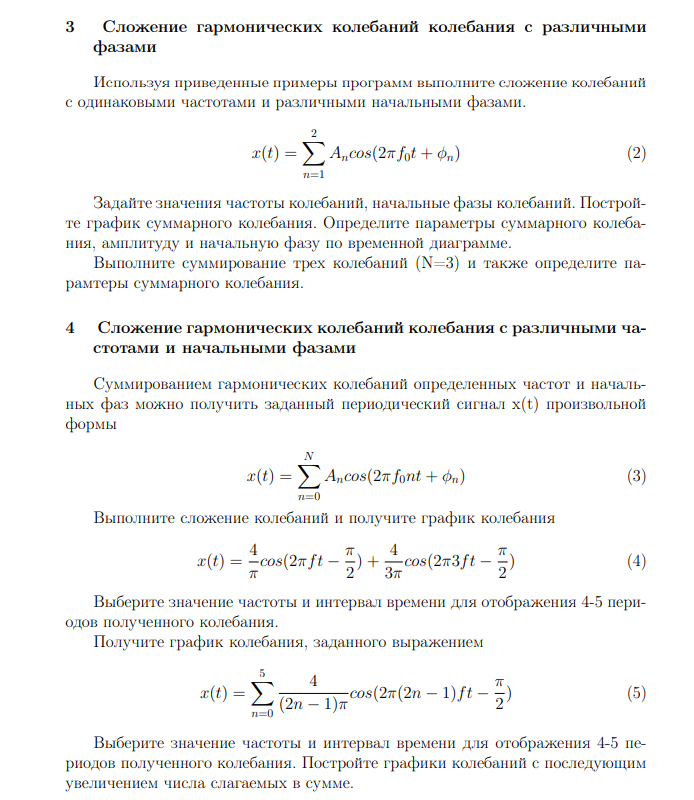
\includegraphics[width=1.0\textwidth]{tasks.png}
    \caption{Варианты заданий}
\end{figure}



\endinput